\chapter{Hardware Model and Implementation}

This chapter details the hardware designed during this Master's thesis to accelerate neural network training. The current hardware implements both training and inference acceleration for the neural network architecture described in section \ref{net-arch}.
\todo[inline]{Refer to github, appendix, and project link}
\section{Specifications}
The hardware model was implemented using a ZedBoard. The ZedBoard is a development board equipped with a Zynq-7000 XC7Z020 SoC. The Zynq series has both a processing system and programmable logic, where the processing system is a ARM Cortex-A9 based processor (hereafter referred to as the ``PS'') and the programmable logic is an Artix-7 series FPGA. Bitstreams for the FPGA were generated using Vivado 2018.3 and PetaLinux boot images for the PS were created using Xilinx SDK. The hardware description language (HDL) code for the project was primarily written in SystemVerilog. The programs run on the PS were written in C.

\section{The Implemented Neural Network}\label{net-arch}
The classical MNIST handwritten digit dataset was chosen as the problem setting for the hardware model as a proof-of-concept. This problem has been chosen to verify the value in designing accelerators that take advantage of the finer-grained parallelism present in neural networks. The network consists of an input layer, 3 fully-connected layers, and a softmax output layer. The input layer is a 28$\times$28 grayscale image of a handwritten digit. The dimensions of the rest of the layers in the network are shown in table \ref{net-arch-table}. Layers whose name starts with FC are fully-connected layers. 
\begin{table}
	\centering
	\begin{tabular}{|c| c| c|}
		\hline
		\textbf{Layer Name}	& \textbf{Input Size} & \textbf{Output Size}\\\hline
		FC0	& 784 (28$\times$28) & 98 \\\hline
		FC1 & 98 & 64 \\\hline
		FC2 & 64 & 10 \\\hline
		Softmax & 10 & 10\\\hline
	\end{tabular}
	\caption{The hidden and output layers in the implemented neural network}
	\label{net-arch-table}
\end{table}

\section{Design Goals}
There were a few key principles that guided the overall design process throughout the development of the hardware accelerator. A core tenet was to maintain the project such that in the future HDL could be generated for training a network of any architecture so long as the desired layer types had an implementation. As a result, all layers have been modularized and internal components are parameterized. Designing in a modular and parameterizable fashion also allows for quick and easy readjustments to the neural network architecture if needed.
\par 
In addition, optimal usage of resources available was prioritized. For example, the limiting FPGA resource was the amount of digital signal processing slices (DSPs). Therefore, the FPGA design optimized the distribution of DSPs over other resources as opposed to saving an extra Block RAM (BRAM) block. 

\section{Overall Architecture}
In the hardware model, both the Zynq's PS and the FPGA were used to facilitate a cohesive and efficient architecture to accelerate neural network computation. The overall system architecture can be seen in figure \ref{overall-arch}. 

Through memory-mapped I/O, the PS transfers neural net hyperparameters, training data, and control signals to the FPGA. The FPGA transfers training statistics and state data back to the PS. The interface is further described in sections \ref{az-com} and \ref{mmio-lay}.

Inside the FPGA, the neural network described in section \ref{net-arch} is implemented. Layers are connected in both forward and backward directions in order to support training. There are three types of primary modules in the top-level of the FPGA: fully-connected layers, interlayer activation buffers, and the softmax layer. In addition, there is a general control flow in the top-level with which all the primary modules interact.

\begin{figure}
	\centering 
	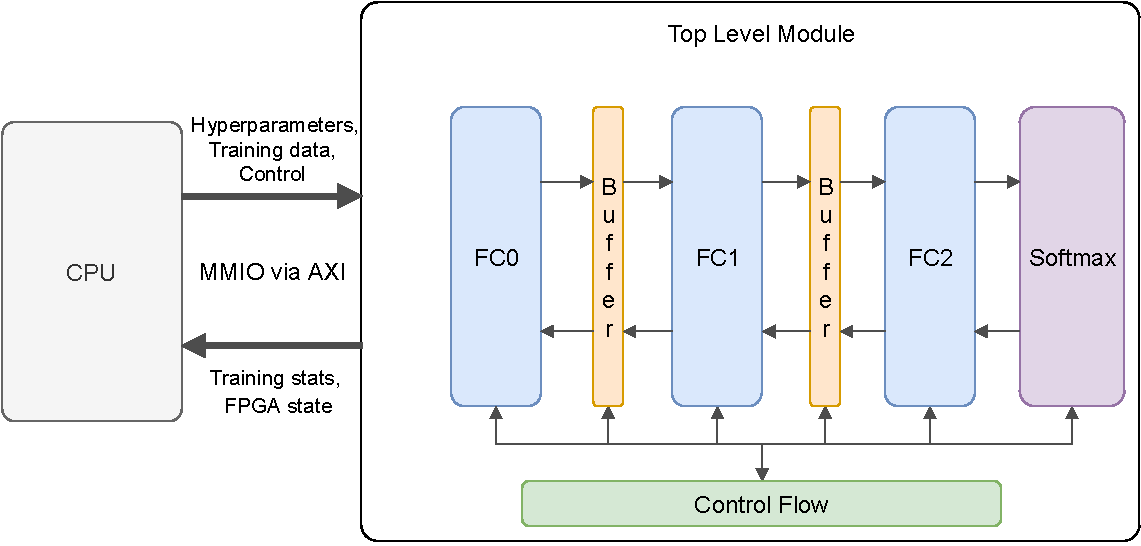
\includegraphics[width=\textwidth]{figures/overall_arch}
	\caption{Architecture of the hardware accelerator}\label{overall-arch}
\end{figure}

\section{Module Architecture}
As mentioned in the design goal section, one of the tenets of this design was to allow for modularity and parameterization, such that changing a network architecture would not require too much work. As such, there are a few global parameters defined, such as the amount of bits specified for the fixed-point precision. There are also parameters defined for each of the fully-connected layers. These parameters can all be found in the \textit{sys\_defs.vh} file in the Appendix \todo[inline]{fpga appendix}, or on GitHub. 


\subsection{Fully-Connected Layers}
The fully-connected layer modules implement both forward and backward passes. The general architecture is shown in figure \ref{fc-arch}. As DSP slices are limited, both the forward and backward computational units make use of the same resources to compute multiplications, known as the kernel pool. There are 4 modes of computation in the fully-connected layer: forward pass, backpropagating neuron gradients, computing weight gradients, and updating the weights. Of these 4 modes of computation, all except updating the weights make use of the kernel pool. This is because updating the weights makes uses of bit shifting instead of multiplication to multiply gradients by the learning rate.
\begin{figure}
	\centering 
	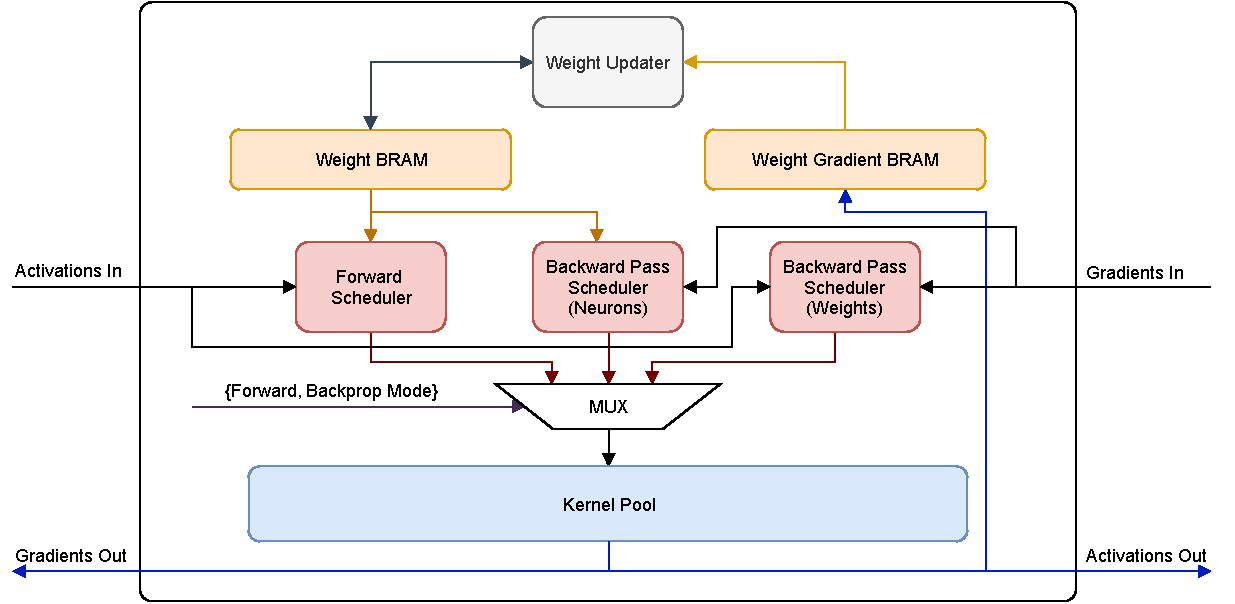
\includegraphics[width=\textwidth]{figures/fully_connected_arch}
	\caption{Architecture of the fully connected layer}\label{fc-arch}
\end{figure}

The forward pass multiplies weights and input activations to produce output activations. Backpropagating neuron gradients multiplies weights by current layer input gradients to produce previous layer gradients as output. The weight gradient computation mutliplies input activation from the forward pass by the current layer gradient, and then writing the computed gradient to the weight gradient BRAM. 

Since being flexible and modular was one of the design goals, all the fully-connected layers use the same kernel and scheduler modules, with different parameters in the instantiation.

\paragraph{Scheduling}
Each of the computational modes needs to have a scheduler to generate addresses to be read and guide the computation. For this, the a generalized scheduler module was implemented. The scheduler uses two pointers starting from the head and middle of the BRAM, and iterates through the entirety during the forward pass. Since the weight BRAMs of each layer are different, certain parameters are assigned for instantiations of the scheduler.	
\paragraph{Kernel}
\begin{figure}
	\centering 
	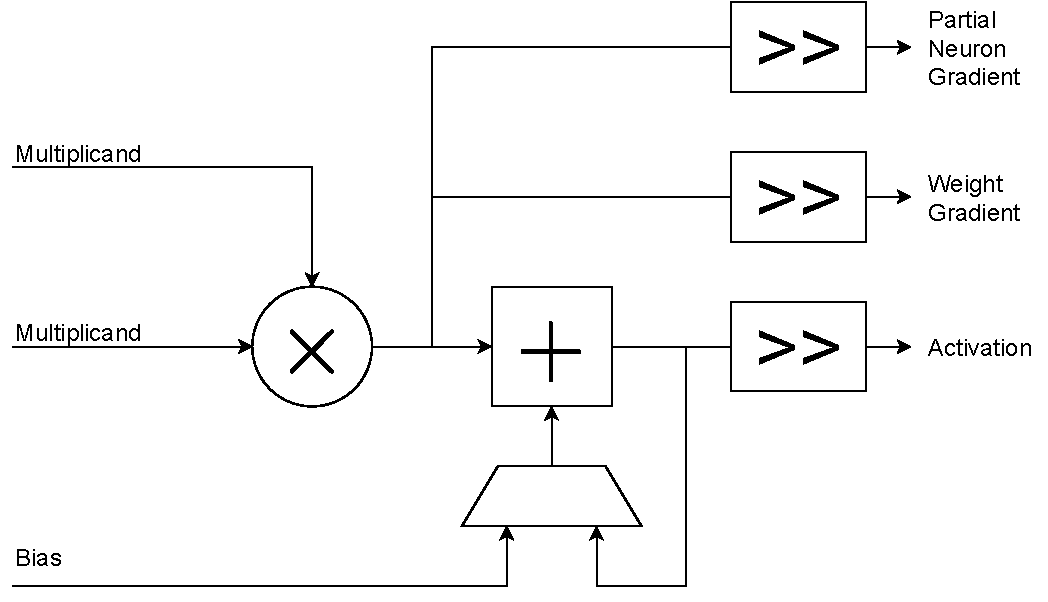
\includegraphics[width=5in]{figures/kernel_arch}
	\caption{Architecture of the kernel}\label{kernel-arch}
\end{figure}
\paragraph{BRAM Layout}
\paragraph{Weight Updates}

\subsubsection{Individual Fully-Connected Layer Implementation}



\subsection{Interlayer Architecture}
\begin{figure}
	\centering 
	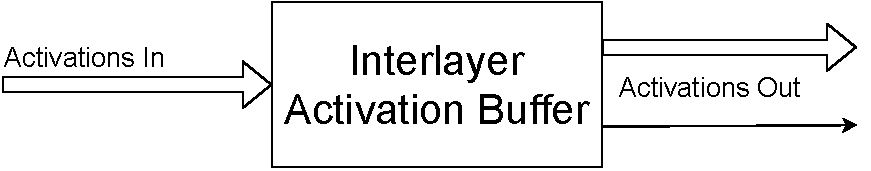
\includegraphics[width=\textwidth]{figures/interlayer_buffer}
	\caption{The interlayer buffer}\label{softmax-arch}
\end{figure}
\subsection{Softmax Layer}
\begin{figure}
	\centering 
	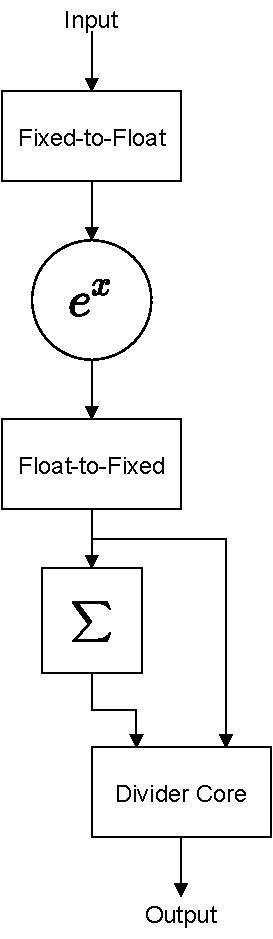
\includegraphics{figures/softmax}
	\caption{Architecture of the softmax layer}\label{softmax-arch}
\end{figure}
To have training be feasible, a proper loss function was required to calculate initial gradients for the output neurons. As such, cross entropy loss, one of the most popular loss functions in deep learning was chosen for this network. Cross-entropy loss is a statistical loss that uses probabilities as input, as shown below.



\begin{align}
\mathcal{L}(y) = - \sum_{i = 1}^{C}y_{i,c}\log(p_{i,c})
\end{align}
In this equation, 
\todo[inline]{Consider against the cross entropy loss defined in chapter 3, define it in chapter 2 IMO}

As explained in chapter \ref{background}, the softmax functions converts logits to probabilities in following manner

\section{ARM-Zynq Communication}\label{az-com}
\section{Memory Map Layout}\label{mmio-lay}
The memory 
\section{Project Structure}


\begin{figure}
	\begin{tikzpicture}[]
	\node[] at (0,0) (top) {neural\_net\_top.sv};
	\node[] at (3, -1) (mlled) {fc0\_layer.sv};
	\node[] at (3, -2) (debounce) {debounce.v};
	\node[] at (3, -3) (scope) {red\_pitaya\_scope.v};
	\node[] at (3, -4) (buffermodule) {buffer\_module.v};
	\node[] at (3, -5) (irf) {internal\_ref\_gen.xci};
	\node[] at (3, -6) (pfd) {pfd.v};
	\node[] at (6, -7) (pfdblock) {pfd\_block.v};
	\node[] at (6, -8) (pfdfilter) {pfd\_filter.v};
	\node[] at (3, -9) (freqcounter) {freq\_counter.v};
	\node[] at (6, -10) (freqcounterblock) {freq\_counter\_block.v};
	\node[] at (9, -11) (interp) {freq\_interp\_clk.xci};
	\node[] at (3, -12) (pid) {red\_pitaya\_pid.v};
	\node[] at (6, -13) (pidblock) {imra\_pid\_block.v};
	\node[] at (6, -14) (pidfilt) {iir\_filter.v};
	\node[] at (3, -15) (analog) {red\_pitaya\_analog.v};
	\node[] at (6, -16) (dds) {dds/mixer/lpf};
	
	
	\draw [->] (top) |- (mlled.west);
	\draw [->] (top) |- (debounce.west);
	\draw [->] (top) |- (scope.west);
	\draw [->] (top) |- (buffermodule.west);
	\draw [->] (top) |- (irf.west);
	\draw [->] (top) |- (pfd.west);
	\draw [->] (top) |- (freqcounter.west);
	\draw [->] (top) |- (pid.west);
	\draw [->] (top) |- (analog.west);
	\draw [->] (pfd) |- (pfdblock.west);
	\draw [->] (pfd) |- (pfdfilter.west);
	\draw [->] (freqcounter) |- (freqcounterblock.west);							
	\draw [->] (freqcounterblock) |- (interp.west);
	\draw [->] (pid) |- (pidblock.west);
	\draw [->] (pid) |- (pidfilt.west);
	\draw [->] (analog) |- (dds.west);
	
	
	
	\end{tikzpicture}
	\caption{Hierarchy of the FPGA code used for the implementation of the network.}
\end{figure}